\section{Design Process or Methodology Overview}

Phase 3 was designed as a controlled comparison of visual representations rather than as a search for a single large architecture. The study first established defensible data partitions, then trained one RGB reference model for each task, and finally evaluated a cattle-centered counterpart under the same task protocol. This sequence produced six completed single-task experiments. The remaining two experiments will compare hard parameter sharing with a modular multi-task design; their results are intentionally excluded from the present manuscript.

The central design variable is the information supplied to each task. BCS depends primarily on morphology, Behavior requires posture together with temporal change, and Re-ID depends on stable individual appearance. The cattle-centered models therefore share a general principle---focus the representation on the target animal---but do not use an identical preprocessing rule. Figure~\ref{fig:phase3design} shows the progression from protected task protocols to the completed task comparisons and the two pending MTL experiments.

\begin{figure}[htbp]
\centering
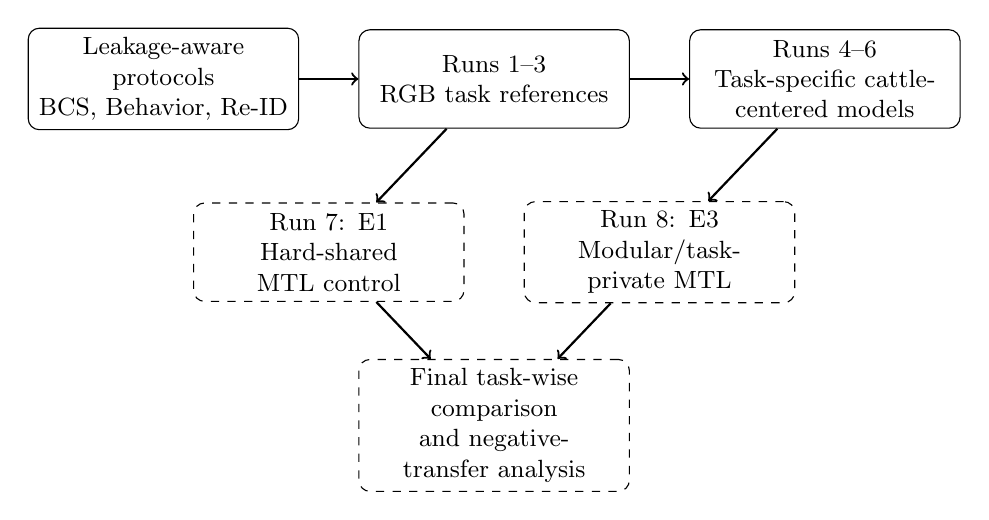
\begin{tikzpicture}[
  box/.style={draw,rounded corners,align=center,text width=3.2cm,minimum height=1.25cm,font=\small},
  pending/.style={box,dashed},
  arrow/.style={->,thick}
]
\node[box] (protocols) at (0,0) {Leakage-aware protocols\\BCS, Behavior, Re-ID};
\node[box] (rgb) at (4.2,0) {Runs 1--3\\RGB task references};
\node[box] (centered) at (8.4,0) {Runs 4--6\\Task-specific cattle-centered models};
\node[pending] (e1) at (2.1,-2.2) {Run 7: E1\\Hard-shared MTL control};
\node[pending] (e3) at (6.3,-2.2) {Run 8: E3\\Modular/task-private MTL};
\node[pending] (synthesis) at (4.2,-4.4) {Final task-wise comparison\\and negative-transfer analysis};
\draw[arrow] (protocols) -- (rgb);
\draw[arrow] (rgb) -- (centered);
\draw[arrow] (rgb) -- (e1);
\draw[arrow] (centered) -- (e3);
\draw[arrow] (e1) -- (synthesis);
\draw[arrow] (e3) -- (synthesis);
\end{tikzpicture}
\caption[Phase 3 comparative research design]{Phase 3 comparative design. Solid boxes are supported by completed Runs 1--6; dashed boxes identify the pending MTL experiments and final synthesis.}
\label{fig:phase3design}
\end{figure}


Table~\ref{tab:runstatus} summarizes the experimental sequence and its current boundary.

\begin{table}[htbp]
\centering\small
\caption[Deadline comparison status]{Deadline comparisons and artifact status at the reviewed snapshot.\evidence{E02,E03,E19,E21}}\label{tab:runstatus}
\begin{tabularx}{\textwidth}{lYY}
\toprule
Run & Role & Status \\
\midrule
1 & BCS RGB & Result recorded; execution revision missing. \\
2 & Behavior single-frame RGB & Result recorded; cache/provenance audit pending. \\
3 & Re-ID RGB & Implemented and smoke-tested; full result pending. \\
4 & BCS cattle-centered & Pending; pose acceptance unresolved. \\
5 & Behavior cattle-centered + TCN & Pending. \\
6 & Re-ID cattle-centered & Pending. \\
7 & Hard-shared MTL (E1) & Pending. \\
8 & Task-conditioned MTL (E3) & Pending; final design not fixed. \\
\bottomrule
\end{tabularx}
\end{table}


Runs 4--6 are combined-configuration comparisons. Run 4 changes localization, cropping, and mask guidance together; Run 5 changes both the spatial representation and temporal aggregation; and Run 6 changes crop geometry and adds an oracle mask channel. Their results measure the complete executed configurations. They do not isolate a causal contribution for any one component.

\section{Preliminary Design or Design (Model) Specification}

\subsection{Representation Alternatives}

The RGB references use ImageNet-pretrained ResNet-18 encoders because this backbone provides a common, computationally manageable starting point across the three tasks~\cite{he2016resnet}. Task-specific heads then reflect the output structure: cumulative ordinal logits for BCS, categorical logits for Behavior, and an identity classifier plus a retrieval embedding for Re-ID. This separation permits a fair question: when the task and evaluation protocol are held fixed, does a cattle-centered input representation provide a more useful feature space than the RGB reference?

Localization and segmentation were selected after a feasibility study of pretrained perception models. The study compared detector return behavior and latency and, where SideView ground-truth masks were available, measured segmentation overlap. RT-DETR-L followed by SAM 2.1 provided a practical automatic pipeline for ScienceDB and Behavior, while SideView enabled a distinct oracle experiment using its released target-cow masks~\cite{zhao2024rtdetr,ravi2024sam2}. Pose outputs were not included in Runs 4--6 because their task relevance and cross-dataset reliability were insufficiently established. Viewpoint was likewise retained as a separate completed study rather than being inserted into downstream models without validated transfer.

\subsection{Run 1: RGB Body Condition Scoring}

The BCS reference uses an ImageNet-initialized ResNet-18 with four independent cumulative threshold logits for five ordered classes. For a class index $y\in\{0,1,2,3,4\}$, the target for threshold $k$ is
\begin{equation}
 t_k=\mathbb{I}(y>k),\qquad k=0,1,2,3.
\end{equation}
If $g_k=\mathbf{w}_k^\top\mathbf{h}+b_k$ is the corresponding logit, the batch loss is
\begin{equation}
 L_{\mathrm{BCS}}=-\frac{1}{4B}\sum_{i=1}^{B}\sum_{k=0}^{3}
 \left[t_{ik}\log\sigma(g_{ik})+(1-t_{ik})\log(1-\sigma(g_{ik}))\right].
\end{equation}
The predicted class counts threshold probabilities above 0.5 and is mapped back to the physical scale:
\begin{equation}
 \hat y=\sum_{k=0}^{3}\mathbb{I}(\sigma(g_k)>0.5),\qquad
 \widehat{\mathrm{BCS}}=3.25+0.25\hat y.
\end{equation}
Although the targets are cumulative, the executed head uses independent ordinal binary cross-entropy. It is therefore described as \texttt{ordinal\_bce}, not as CORAL, whose rank-consistency mechanism is different~\cite{coral2020}. The model was trained for 30 epochs with batch size 64, AdamW, an initial learning rate of $10^{-4}$, weight decay $10^{-4}$, a cosine schedule, and seed 42. The checkpoint with the lowest validation MAE was retained.\evidence{E08,E10,E14}

\subsection{Run 4: Cattle-Centered Body Condition Scoring}

Run 4 applies an automatic cattle-centered pipeline to ScienceDB. RT-DETR-L detects COCO cattle at confidence 0.25 or above. When several cattle are returned, the largest bounding box is selected, with confidence used as a tie-breaker. The selected box is expanded by 5\% in each dimension, clipped to the image boundary, and used both as the RGB crop and as the prompt region for SAM 2.1. Images without a valid detection or segmentation are recorded as perception failures and excluded rather than replaced by fabricated inputs.\evidence{E24,E25}

The retained RGB crop and binary mask are resized synchronously to $224\times224$. RGB channels receive ImageNet normalization; the mask remains an unnormalized binary channel in $\{0,1\}$. The ResNet-18 first convolution is expanded from three to four channels. Its RGB weights are copied from the pretrained model, and the additional channel is initialized from the mean of the RGB filters. The ordinal head, target encoding, loss, training schedule, and augmentation policy otherwise follow Run 1. This adds 3,136 trainable parameters, from 11,178,564 to 11,181,700. The executed configuration is therefore a localized RGB crop with explicit binary mask guidance, not a calibrated soft-mask model.\evidence{E24,E25}

\subsection{Run 2: Single-Frame RGB Behavior Recognition}

The Behavior reference uses one representative midpoint frame for each canonical sample and an ImageNet-pretrained ResNet-18 with a five-class linear classifier. The output classes are Standing, Lying, Feeding, Drinking, and Walking, optimized with cross-entropy. CVB samples use the target tracklet information supplied by the dataset, while Kaggle Beef clips already contain one principal animal. The selected checkpoint is epoch 25 of the 30-epoch run, based on validation Macro-F1.\evidence{E05,E09,E12,E15}

This reference deliberately omits temporal aggregation. Its purpose is not to represent the strongest possible video model, but to establish how far a single RGB observation can support the shared five-class taxonomy. The evaluation therefore reports balanced and class-specific measures in addition to pooled accuracy, particularly because Walking occurs only in CVB.

\subsection{Run 5: Cattle-Centered Temporal Behavior Recognition}

Run 5 replaces the midpoint image with eight approximately evenly spaced observations from the labeled interval. Its input tensor has shape $[B,8,4,224,224]$. Each time step contains an RGB crop and a binary mask. For CVB, the exact target-tracklet bounding box at the sampled frame prompts SAM 2.1; the same coordinates crop RGB and mask. No nearest-animal or full-frame substitution is permitted. For the single-cow Beef clips, RT-DETR-L supplies the principal cow box when possible, followed by a positive center prompt to SAM 2.1; an image-center prompt is used when the detector returns no cow. A sequence is excluded if any required mask is empty or invalid.\evidence{E26,E28}

The completed Train/Validation cache retained 4,271 of 4,465 candidate sequences: 3,641 for training and 630 for validation. It contains 34,168 authentic RGB frames and 34,168 non-trivial binary masks. The 194 exclusions were recorded as empty-mask failures; all 145 Walking candidates across Train and Validation were retained. The held-out test comparison separately retained 780 of 809 samples, consisting of 422 CVB and 358 Beef sequences.\evidence{E26,E27}

Each frame is encoded by a four-channel ResNet-18 into a 512-dimensional feature. The resulting sequence $\mathbf{H}\in\mathbb{R}^{B\times8\times512}$ is transposed for temporal convolution. The first temporal block uses a width-three Conv1D projection from 512 to 256 channels, BatchNorm, GELU, dropout 0.2, and a width-one residual projection. A second width-three 256-channel block applies the same normalization, activation, and dropout with an identity residual. Adaptive average pooling over time produces one 256-dimensional vector, followed by the five-class linear head. This is a lightweight residual Conv1D aggregator over sparsely sampled features; it is not optical flow, a video transformer, or a deep dilated causal TCN. The complete model has 11,903,621 trainable parameters.\evidence{E28}

\subsection{Run 3: RGB Cattle Re-Identification}

The Re-ID reference follows SideView Protocol A. Representation learning uses 41 parlor-only cows, restricted to 12,753 training and 2,683 validation images. Evaluation uses 69 different cows: a 36,811-image parlor gallery, 25,260 barn queries for all 69 cows, and 607 snapshot queries for 63 of them. The representation-learning and evaluation identities are disjoint.\evidence{E06,E20,E22,E23}

ResNet-18 produces a raw 512-dimensional feature $\mathbf{h}$. A 41-class linear classifier is trained on the raw feature using cross-entropy, while retrieval uses its L2-normalized form:
\begin{equation}
 \mathbf{z}=\frac{\mathbf{h}}{\lVert\mathbf{h}\rVert_2},\qquad
 \boldsymbol{\ell}=W\mathbf{h}+\mathbf{b}.
\end{equation}
At evaluation, cosine similarity is computed as the dot product between normalized query and gallery embeddings. Gallery images are ranked for each query, and the evaluation reports Rank-$k$ retrieval and mean average precision (mAP). The full model was trained for 30 epochs; the validation-selected representation was then evaluated once on the held-out Protocol A conditions.\evidence{E20,E22,E23}

\subsection{Run 6: Oracle Segmentation-Guided Re-Identification}

Run 6 uses SideView's released target-cow masks and is therefore an oracle GT segmentation-guided experiment. The non-zero mask region defines a bounding box, which is expanded by approximately 5\%. Identical coordinates crop RGB and mask before both are resized to $224\times224$. RGB is ImageNet-normalized, the mask remains binary $\{0,1\}$, and RGB is not multiplied by the mask. The first ResNet convolution is expanded to four channels with the mask filters initialized from the mean RGB weights. All other representation-learning and retrieval procedures remain aligned with Run 3.\evidence{E29,E30}

This design tests whether reliable target-centered geometry and explicit foreground guidance improve cross-setting retrieval. It does not validate an automatic segmentation pipeline, and it does not separate the effect of cropping from the effect of the fourth channel. The parameter change is limited to 3,136 weights, increasing the trainable count from 11,197,545 to 11,200,681.\evidence{E29,E30}

\section{Data Collection and Preparation}

\subsection{Data Sources and Scientific Roles}

All experiments use existing datasets; no new farm data collection is claimed. ScienceDB is the primary BCS source, CVB plus Kaggle Beef forms the primary Behavior stack, and SideViewCows2026 is the primary Re-ID benchmark. External sources have predefined stress-test roles but are not reported as evaluated without result artifacts. Table~\ref{tab:datasets} separates these roles.

\begin{table}[htbp]
\centering\small
\caption[Dataset roles and interpretation boundaries]{Current dataset roles and interpretation boundaries. Counts are project records, not raw-data verification in this writing environment.\evidence{E04,E05,E06,E07}}\label{tab:datasets}
\begin{tabularx}{\textwidth}{lYY}
\toprule
Source & Role / scale & Boundary \\
\midrule
ScienceDB & Primary BCS; 53,566 RGB images & 5,653 burst groups; no verified biological IDs. \\
CVB + Beef & Primary Behavior; 5,274 rows & Source/session groups; five mapped classes. \\
SideView & Primary Re-ID; 80,260 image/mask pairs; 110 cows & Named recording/identity protocols. \\
Ruchay / Dryad & External BCS & Score support, scale and modality differ. \\
MmCows / CBVD-5 & External Behavior & Label and temporal compatibility must be checked. \\
BECA-L / BECA-D & External Re-ID stress tests & No retrieval results claimed. \\
MultiCam / OpenCows & Blocked / legacy & Neither is the active primary. \\
\bottomrule
\end{tabularx}
\end{table}


ScienceDB contains 53,566 RGB images over five scores from 3.25 to 4.25. The released metadata do not provide verified biological cow identities. Its 5,653 repaired connected burst groups are therefore the strongest defensible separation unit. ScienceDB results are described as burst-group-disjoint, passage-disjoint, or sequence-safe, never as unseen-cow evaluation.\evidence{E04}

The Behavior manifest contains 2,481 CVB segments and 2,793 Beef clips. CVB is grouped by source video, and Beef by recording session/source-video provenance. The combined dataset has 267 protected groups and 5,274 samples. Because Walking is supplied only by CVB, the primary test is source/session-group-disjoint but not cow-disjoint, and pooled accuracy alone is insufficient.\evidence{E05,E13}

SideView contains 80,260 RGB images, 80,260 paired binary masks, and 110 biological identities. Protocol A deliberately separates 41 representation-learning cows from 69 evaluation cows. It therefore supports an identity-disjoint statement for Runs 3 and 6, unlike the BCS and Behavior protocols.\evidence{E06}

\subsection{Label Harmonization and Split Protection}

ScienceDB labels retain their physical BCS values. CVB labels are mapped from resting-standing, resting-lying, grazing, drinking, and walking to the five canonical classes; Beef contributes stand, lie, eat, and drink, while rumination is excluded. The mapping is fixed before model evaluation. SideView identities are used only within their defined representation-learning or evaluation role.

\begin{table}[htbp]
\centering\small
\caption[Canonical baseline split sizes]{Canonical BCS and Behavior split units.\evidence{E04,E05}}\label{tab:splits}
\begin{tabular}{llrl}
\toprule
Source & Partition & Examples & Groups \\
\midrule
ScienceDB & Train & 37,045 & 3,958 bursts \\
ScienceDB & Validation & 8,481 & 850 bursts \\
ScienceDB & Test & 8,040 & 845 bursts \\
CVB + Beef & Train & 3,785 & 184 source/session \\
CVB + Beef & Validation & 680 & 39 source/session \\
CVB + Beef & Test & 809 & 44 source/session \\
\bottomrule
\end{tabular}
\end{table}


Split protection follows the strongest available provenance. ScienceDB keeps connected burst groups intact. CVB keeps every segment from a source video in one partition, and Beef keeps every derived clip from a recording session in one partition. SideView Protocol A separates cow identities between learning and evaluation and defines acquisition setting explicitly for the gallery and query sets. Under the implemented checks, no forbidden group or identity overlap was detected. This does not justify a universal claim that every possible form of leakage has been eliminated.

\subsection{Perception Feasibility and Component Selection}

The preliminary perception audit compared several off-the-shelf components before they were adopted. It distinguished an output-return rate from accuracy and used mask overlap only where ground truth existed. The results supported RT-DETR-L and SAM 2.1 as practical components, but they also showed that successful inference alone does not guarantee task-relevant anatomy.\evidence{E11}

\begin{table}[htbp]
\centering\small
\caption[Selected perception feasibility results]{Feasibility measurements; detection and pose return rates are not accuracy.\evidence{E11}}\label{tab:perception}
\begin{tabularx}{\textwidth}{lYY}
\toprule
Candidate & Sample / measure & Result \\
\midrule
YOLOv8s & 300 images; any cow returned & 223/300; median 24.5 ms \\
Faster R-CNN v2 & Same detection measure & 285/300; median 470.8 ms \\
RT-DETR-L & Same detection measure & 283/300; median 94.3 ms \\
RT-DETR + SAM 2.1 & 100 SideView images; mask overlap & Mean IoU 0.9216; Dice 0.9530 \\
Oracle box + SAM 2.1 & Ground-truth-derived prompt & Mean IoU 0.9468; diagnostic \\
Pose backbones & 300 images each; output return & 243/300; not pose accuracy \\
\bottomrule
\end{tabularx}
\end{table}


Pose was excluded from the deadline task models after restricted manual review found unreliable ScienceDB rear-view outputs and a landmark schema that did not directly capture the intended BCS anatomy. A separate real-cattle viewpoint classifier later achieved 86.26\% accuracy, 84.96\% balanced accuracy, and 0.8573 Macro-F1 on its own 131-image held-out test. It was not added to Runs 4--6 because transfer to those task datasets was not validated; camera identity was not used as a substitute for viewpoint.\evidence{E31}

\section{Implementation of Selected Design}

Training and preprocessing were implemented in PyTorch, Torchvision, OpenCV, and the Ultralytics perception interface. Deterministic CSV manifests define task samples and partitions. Checkpoints were selected using validation data, and the held-out task tests were evaluated after model selection. Machine-readable artifacts preserve test metrics, confusion matrices, coverage counts, and, where available, split hashes and checkpoint-reload checks.

The local GTX 1050 Ti was restricted to path checks, tensor/loss/metric tests, very small runs, and checkpoint verification. Heavy cache generation, full training, and final task evaluation were executed on Modal cloud GPUs. The unusable RTX 5090 research PC was not used for Phase 3 training. These choices reflect the available compute constraints and separate low-cost validation from production-scale execution.

\subsection{Evaluation Metrics}

BCS is evaluated with physical-score MAE, exact accuracy (Acc@0), accuracy within one adjacent class or $\pm0.25$ BCS units (Acc@1), balanced accuracy, and Macro-F1. For $N$ samples,
\begin{equation}
 \mathrm{MAE}_{\mathrm{BCS}}=\frac{1}{N}\sum_{i=1}^{N}|s_i-\hat{s}_i|.
\end{equation}

Behavior evaluation reports overall accuracy, balanced accuracy, Macro-F1, per-class precision/recall/F1, and source-specific metrics. Balanced accuracy is the mean recall across the five classes and is especially important when class frequencies and source coverage differ.

For Re-ID, Rank-$k$ is the proportion of queries for which at least one correct identity occurs within the first $k$ ranked gallery images. Average precision summarizes the ranking for one query, and mAP averages this value over all queries. Barn-to-Parlor and Snapshots-to-Parlor are reported separately because they represent different acquisition shifts.

\subsection{Planned Multi-Task Integration}

Run 7 will serve as the E1 hard-shared control. Its scientific role is to test whether extensive sharing across BCS, Behavior, and Re-ID creates negative transfer relative to matched single-task references. Run 8 will evaluate the E3 modular alternative, in which task-private processing or adapters/gates permit specialization while retaining a unified framework.

The task datasets do not provide all three labels for the same image. The final implementation must therefore use task-specific batches or an equivalent available-label mechanism and must never interpret an absent annotation as a negative label. Exact sharing boundaries, task sampling, temporal handling, loss weighting, capacity, and compute will be documented from the executed code after Runs 7 and 8 are complete. No comparative MTL result is asserted in this chapter.
